\begin{spacing}{2}
The system design of a testbed for aerial robotic swarms in the given timeframe involved many independent sub-systems to be developed. An incremental yet rapid prototyping approach, as depicted in Fig. \ref{fig:sysdesign}, was followed for development of a Multi-rotor unmanned aerial vehicle which could be used in both indoor and outdoor case scenarios with intra-swarm communication capabilities. The high level system requirements were analysed and sub-systems identified, and developed in parallel. The subsystems so developed were individually tested and integrated into the final design.
\begin{figure}[h]
    \centering
    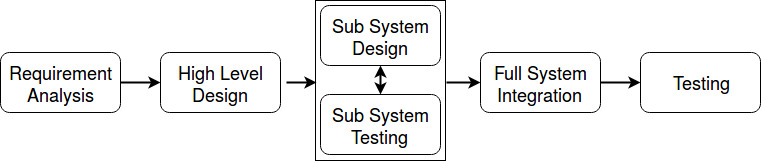
\includegraphics[width = \linewidth]{image/Major_sysdes.jpg}
    \caption{System Design Approach}
    \label{fig:sysdesign}
\end{figure}
\section{System Architecture}
The overall system architecture required for a aerial swarm can be divided into two parts:

\subsubsection*{On-board system}
The on-board system comprises of the following components present on the aerial vehicle:
\begin{enumerate}
\item A fully autonomous unmanned aerial vehicle capable of autonomous flight and navigation using flight controller, localisation unit (GPS), propulsion system, telemetry and RC receiver.
\item Intraswarm communication module capable of handling Ad-hoc network and exchanging current state of the vehicles.
\item An on-board computer capable of communicating with the flight controller and the intraswarm communication module.
\end{enumerate}

\noindent The on-board system architecture is depicted in Fig \ref{fig:sysarch}
\begin{figure}[h]
    \centering
    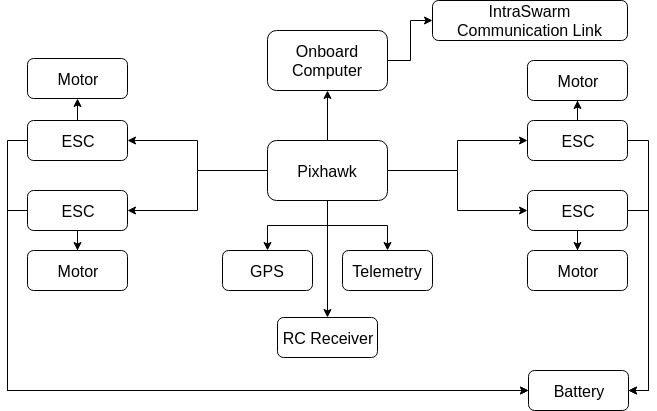
\includegraphics[width=\linewidth, height = 7cm]{sysarc_1.jpg}
    \caption{On-board System Architecture}
    \label{fig:sysarch}
\end{figure}
\subsubsection*{Ground Control System}
The ground control system comprises of a computer with telemetry communication units and a ground station software capable of handling and commanding multiple vehicles. Another computer is used to remote-logging into the on-board computer for running the predefined scripts for communication and running different missions.

\section{Autopilot}
An autopilot is a software stack that uses the information from the sensors connected to a flight controller and the desired mission information to guide the vehicle from one point to the other using the actuators connected to the flight controller. A flight controller is a micro computer hardware with various sensors, actuators and motor drivers connected to it for detecting the current state of the vehicle and controlling it. There exist a number of hobby-grade autopilot stacks and most of the flight controllers come with software already loaded that has an autopilot function.

\subsection{ArduPilot}
\textit{ArduPilot is an open source, unmanned vehicle Autopilot Software Suite, capable of
controlling autonomous}:
\begin{itemize}
    \item Multirotor drones
    \item Boats
    \item Fixed-wing and VTOL aircraft 
    \item Submarines 
    \item Helicopters
    \item Antenna trackers
    \item Ground rovers
\end{itemize}

ArduPilot which was initially developed as a hobby grade autopilot has evolved to a full-featured autopilot and is being used by professionals in the industry, researchers, as well as amateurs. It's extensive usage can be owed to the growing community of developers that have ensured that ArduPilot consists of all the features and libraries required by any roboticist working in the corresponding field. Ardupilot's source code is stored and managed on GitHub. The navigation software present in the ArduPilot is known as firmware when it is compiled to binary form for micro-controller hardware targets, it runs on vehicles such as copter, plane, rover, antenna tracker and subs. The ground controlling station software includes Mission Planer, APM Planner, QGroundControl, MavProxy.

\subsection{Off-board Control}
Off-board control of an autonomous vehicle involves controlling the flight behaviour by providing actuation commands or lowlevel targets in \textbf{Guided} mode using a computer (on-board or ground based) in the form of mavlink messages over telemetry or serial connection. The system suggested in this report uses Ardupilot software stack for flight controller which allows the multi-rotor to receive commanded linear and angular velocities in all three axis from an on-board computer over serial connection.

\section{Communication System}
The proposed system requires communication between multiple vehicles and between each vehicle and ground station. The required communication can be divided into 3 categories as follows:
\begin{itemize}
    \item \textbf{Telemetry} connection between vehicle and ground control station.
    \item \textbf{Remote control} communication to ensure safety in case of unexpected behaviour.
    \item \textbf{Intra-swarm} communication to transfer information between vehicles for coordination.
\end{itemize}

\noindent Due to the presence of plenty of custom off the shelf (COTS) telemetry and remote control modules in the market, we only cover the \textbf{intra-swarm} communication module in detail. 
\subsection{Intra-Swarm Ad-Hoc Network}
The intra swarm communication module requires efficient and real-time transfer of state of a UAV to all other vehicles in the swarm in order to maintain coordination and avoid collisions. Since each vehicle requires information of every vehicle in its neighbourhood, we need a mesh topology. Also, the author chose to use Ad-hoc network instead of a centralised station and access point approach to ensure the crash of one vehicle doesnt render the rest of the swarm useless.


A decentralised network that does not rely on pre-built infrastructure or devices such as routers and access points is known as an ad-hoc network. WANET i.e. wireless ad-hoc network and MANET i.e. mobile ad-hoc network are commonly used ad-hoc networks. Ad-hoc networks do not require a connection with a ground control station and the messages are transferred between individual nodes directly. It relies on a set of routing algorithms that dynamically determine the flow of messages between the nodes depending on the connectivity, traffic and cost of transfer of messages. However, essential information is shared with the ground control station with the help of "star" approach where in the individual nodes that is the UAVs in our case take turns to transfer information to the ground control station. An ad-hoc network is an essential requirement of swarm of robots to ensure that the whole swarm system is not affected by the failure, removal or addition of nodes. This feature will make the swarm system more flexible and reliable. Ad-hoc networking allows local information sharing and distributive decision making which makes the swarm capable of resolving a problem in the most efficient and effective way.

Ad-Hoc networks, being self-configuring in nature, allow devices to create and join networks "on the fly". With wireless ad-hoc networks embedded in UAVs, multiple UAVs can work collaboratively like a team to complete a task.

%A wireless ad hoc network[1] (WANET) or MANET (Mobile ad hoc network) is a decentralised type of wireless network.[2][3] The network is ad hoc since it does not require any pre-existing infrastructure, such as routers in wired networks or access points in managed (infrastructure) wireless networks.[4] Instead, data is forwarded by each node to the neighbours. The routing algorithm and the network connectivity are used to dynamically decide which node will be forwarding data.[5]
%In the Windows operating system, ad-hoc is a communication mode (setting) that allows computers to directly communicate with each other without a router.
%Wireless mobile ad hoc networks are self-configuring, dynamic networks in which nodes are free to move. Since Wireless networks lack the complexities of infrastructure setup and administration, it enabling devices to create and join networks "on the fly" – anywhere, anytime.[6]
% With wireless ad hoc network technology embedded into the UAVs, multiple UAVs can communicate with each other and work as a team, collaboratively to complete a task and mission. If a UAV is destroyed by an enemy, its data can be quickly offloaded wirelessly to other neighboring UAVs. The UAV ad hoc communication network is also sometimes referred to UAV instant sky network. 
%Robots are mechanical systems that drive automation and perform chores that would seem difficult for man. Efforts have been made to co-ordinate and control a group of robots to undertake collaborative work to complete a task. Centralized control is often based on a "star" approach, where robots take turns to talk to the controller station. However, with wireless ad hoc networks, robots can form a communication network on-the-fly, i.e., robots can now "talk" to each other and collaborate in a distributed fashion.[33] With a network of robots, the robots can communicate among themselves, share local information, and distributively decide how to resolve a task in the most effective and efficient way.[34]


\section{ROS Architecture}
Robotics Operating System is an open-source, meta-operating system for robotics
applications. Despite not being a complete operating system, it provides services like
hardware abstraction, low-level device control, implementation of commonly-used
functionality, message-passing between processes, and package management which
are usually found in a completely developed operating system. ROS also provides
tools and libraries for obtaining, building, writing, and running code across multiple
computers. Despite the importance of reactivity and low latency in robot control, ROS
itself is not a real-time OS (RTOS). It is possible, however, to integrate ROS with
real-time code.
Use of ROS architecture allows easy scaling up of the swarm and provides an easy
to use and highly accessible interface to users for testing new algorithms rapidly.
\subsection{MAVLink ROS Bridge}
MAVlink is the communication protocol developed for sending and receiving
messages from micro autonomous vehicle to ground control station (laptop). The
library has been around since 2009 and is supported and used by more than 95\% of
open-source flight firmwares and ground control station softwares. Since the autopilot
can only respond to mavlink commands, it is necessary to create a mavlink to ros
bridge to account for the high level of computational requirements for running
multiple algorithms.
The MAVLink ROS interface is provided by the MAVROS package developed by
Vladimir Ermakov for ROS Indigo.\cite{mavros}

The open-source ROS package however has
support for connecting only 1 vehicle at a time. The package provides interface to
current state of the system in the form of topics which can be subscribed to using
other nodes to work upon this data. Other topics like setpoint wait for ROS nodes to
publish data to act upon. Other features like mode change and arming/disarming are
provided by the use of services. The position of vehicle in the local frame can be
accessed using /mavros/local\_position/pose topic or /mavros/global\_position/global to
access GPS coordinates.

The MAVROS package was changed in order to allow multiple vehicles to connect
to itself by making the use of namespaces. Namespaces act like a mask in order to
change the name of any ROS node, topic or service. Namespaces were utilised to
avoid the problem of overriding names when running multiple MAVROS instances.
All the topics, nodes and services related to mavros have the common ‘/mavros/..’
keyword at the beginning of their names. Thus, launching multiple MAVROS
instances forced the names of two or more entities to be same causing the ROS master
to crash. The problem was solved by renaming the nodes, topics and services to
“/id/mavros/..” which not only helped solve the override problem but also allowed
easier identification and differentiation of vehicles.
The topics used for the purpose of localisation and control of multi-rotor are as
follows:
\begin{itemize}
    \item /id/mavros/local\_position/pose
    \item /id/mavros/global\_position/global
    \item id/mavros/VFR\_Hud
    \item id/mavros/setpoint\_velocity/cmd\_vel
\end{itemize}

Various other services have also been used to change mode of operation of vehicle
and to arm and disarm the vehicles.
Fig. \ref{fig:rqtgraph} shows the graph of major topics and nodes being used
by three vehicles sharing a common swarm architecture.

\begin{figure}
    \centering
    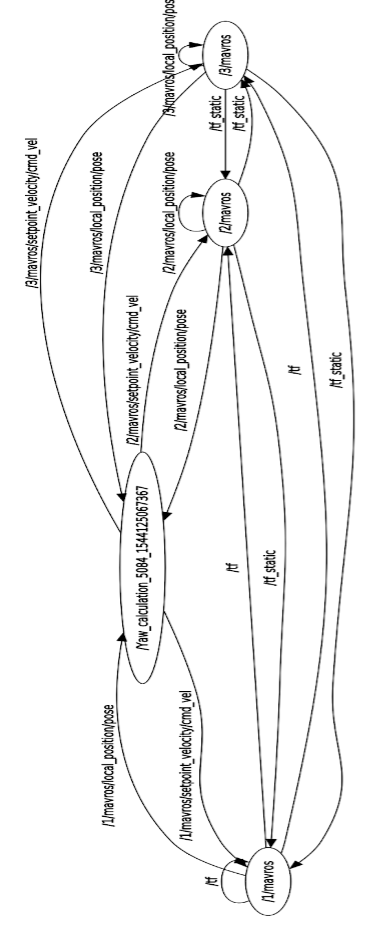
\includegraphics[height = 9in]{image/rqt_plot.png}
    \caption{Communication Node graph for three vehicles}
    \label{fig:rqtgraph}
\end{figure}

\end{spacing}